\documentclass[11pt]{article}
\usepackage{geometry}                % See geometry.pdf to learn the layout options. There are lots.
\geometry{a4paper}                   % ... or a4paper or a5paper or ... 
%\geometry{landscape}                % Activate for for rotated page geometry
%\usepackage[parfill]{parskip}    % Activate to begin paragraphs with an empty line rather than an indent
\usepackage{graphicx}
\usepackage{amssymb}
\usepackage{epstopdf}
\DeclareGraphicsRule{.tif}{png}{.png}{`convert #1 `dirname #1`/`basename #1 .tif`.png}
\usepackage{tabularx}
\usepackage{url}
\usepackage[french]{babel}	%francais
\usepackage[latin1]{inputenc}	%francais
\usepackage{xspace} %pour les guillemets franÁais : \og coucou \fg
\usepackage[french, vlined, ruled]{algorithm2e}

\newcommand{\cad}{c'est-‡-dire~}
\title{
\LARGE{\'Etude d'un langage de description des propriÈtÈs temporelles d'une architecture et d'un outil de gÈnÈration de simulateur temporel.}\\\LARGE{$\star$}\\
\Large{PrÈsentation des choix techniques}
\\
\large{Projet MasCotTE, lot ‡ T0+9 de la t‚che 1.3}
%Projet soutenu par l'ANR
}
\author{MikaÎl Briday, Jean-Luc BÈchennec et Yvon Trinquet \\ IRCCyN \\ BP 92101 \\ 1, rue de la NoÎ \\ 44321 Nantes cedex 3}
\date{}                                           % Activate to display a given date or no date

\begin{document}
\maketitle
~
\newpage
~
\newpage
\tableofcontents
\newpage
\section{Introduction}

%provenance directe du fichier Mascotte -> Base de l'intro.
L'objectif, global et final, de l'�tude est l'obtention par une technique de simulation, du WCET d'un code ex�cutable. La simulation concerne l'ex�cution d'un code sur une architecture mat�rielle monoprocesseur ou multiprocesseurs (n{\oe}uds en r�seau, CAN par exemple). L'architecture mat�rielle comprend les processeurs et les p�riph�riques associ�s (cas des micro-contr�leurs), y compris les contr�leurs r�seaux. Le code �tant connu le probl�me est la simulation r�aliste de l'architecture mat�rielle, donc entre autres la simulation r�aliste du processeur. L'inconv�nient majeur d'une telle approche, trait�e de fa�on classique, est que tout changement de processeur n�cessite de refaire le simulateur, ce qui est complexe et co�teux en temps. C'est pourquoi l'approche propos�e est fond�e sur les langages de description d'architecture mat�rielle. 

Un langage de description d'architecture mat�rielle permet de d�crire tout ou partie des diff�rents  composants mat�riels qui forment un calculateur, voire un ensemble de calculateurs communiquant au  travers d'un r�seau. Traditionnellement les langages de description d'architecture se sont focalis�s, d'une 
part sur la description du jeu d'instructions du microprocesseur et de l'architecture associ�e (� condition que cette architecture reste simple), et d'autre part sur l'exploration de l'espace de conception (\textsl{Design Space Exploration}) avec l'objectif de produire un simulateur du processeur et des outils logiciels comme un assembleur et un compilateur. On peut citer nML, LISA ou encore eXPression. La description de la hi�rarchie m�moire est  assez peu abord�e, les aspects r�seau et utilisation de processeurs h�t�rog�nes pas du tout. De plus, le noyau d'ex�cution le plus sophistiqu� qu'il est possible de d�crire consiste en un pipeline.  Le contexte o� nous nous pla�ons est diff�rent puisqu'il s'agit de d�crire des processeurs existants ainsi  que les p�riph�riques associ�s (orientation marqu�e vers les microcontr�leurs) afin de : 
\begin{itemize}
\item disposer d'une description incluant des param�tres temporels pour alimenter des outils de placement, de validation ou de  calcul du WCET ;
\item g�n�rer un simulateur automatiquement � partir de la description de l'architecture. 
\end{itemize}

Un tel simulateur peut alors �tre int�gr� au sein d'une plate-forme logicielle utilis�e pour la mise au point,  le d�bogage et le test des programmes temps r�el ou encore, comme c'est le cas ici, dans la plateforme OTAWA pour permettre l'�valuation du WCET sur du code ex�cutable. Par ailleurs, contrairement aux 
langages existants qui se focalisent sur la description structurelle, ce langage prendrait principalement en  compte la description temporelle. D�crire l'architecture au moyen d'un langage d�di� pr�sente plusieurs avantages : la mise en {\oe}uvre et les  modifications de la plate-forme sont plus rapides et la mise au point du simulateur, dans la mesure o� il  peut �tre g�n�r� automatiquement, est aussi plus rapide puisqu'une v�rification de la coh�rence de  l'architecture peut �tre faite � partir de la description.  Il s'agit donc d'�tudier un  langage et les mod�les associ�s afin de d�crire des architectures complexes 
incluant la hi�rarchie m�moire, les bus, les r�seaux de communication, etc. du point de vue fonctionnel,  structurel et temporel. Les simulateurs g�n�r�s utiliseront SystemC (un standard actuel pour la simulation)  et offriront un support pour le test et le d�bogage de haut niveau (t�ches et communication) et bas niveau  (instructions et mat�riel).  Cette proposition s'appuie sur l'expertise de l'IRCCyN dans le domaine (d�veloppement de l'outil ReTiS  de validation d'architecture op�rationnelle par simulation fine, construit autour de l'Infineon C167 avec contr�leur CAN). 






\section{\'Etat de l'art}
Un ADL ou \og Architecture Description Language \fg est un moyen de description commun � l'architecte mat�riel et au concepteur d'outils pour une m�me architecture. Le premier facteur ayant favoris� le d�veloppement des langages ADLs est l'av�nement des ASIPs (Application-Specific Instruction set Processors ). Le second facteur est l'int�r�t grandissant pour les DSPs (Digital Signal Prosessors ) ainsi que pour les SoCs (System-on-Chips).

Des langages tels que VHDL ou VERILOG permettent d�j� de d�crire des architectures mat�rielles. Cependant, un ADL se situe � un niveau d'abstraction plus �lev� et permet:
\begin{itemize}
\item la v�rification sur l'architecture;
\item des modifications rapides sur l'architecture ou le jeu d'instruction pour �valuer les performances (pour l'exploration mat�rielle lors de la phase de conception : \emph{Design Space Exploration});
\item une description plus rapide d'un processeur;
\item l'obtention d'un mod�le de processeur plus rapide (le niveau de finesse est moins �lev�, on ne mod�lise pas forc�ment tous les bus).
\end{itemize}
Les outils qui peuvent �tre g�n�r� de mani�re automatique peuvent �tre un simulateur du processeur, mais aussi l'assembleur, l'�diteur de liens, l'assembleur et le d�boggueur.

\subsection{Classification des ADL mat�riel}
Parmi les ADLs les plus connus, nous citerons ISDL\cite{main97ISDL}, nML \cite{Rajesh99}, MIMOLA\cite{Leupers98}, LISA\cite{zivojnovic96lisa,pees99lisa} et EXPRESSION\cite{halambi99expression}. D'autre part, ces ADLs sont class�s en trois cat�gories:
\begin{description}
\item[ADLs orient�s jeu d'instruction]  Cette cat�gorie se focalisent sur les aspects jeu d'instruction (nML et ISDL par exemple).. L'objectif annonc� de ce type d'ADL est de fournir un compilateur ou/et un simulateur de type ISS\footnote{Instruction Set Simulator. Simulateur fonctionnel, non pr�cis temporellement}. Il n'est pas possible de r�aliser un simulateur temporel en ayant uniquement des informations sur le jeu d'instruction;
\item[ADLs orient�s structure interne ou exploration] Cette cat�gorie va plut�t d�crire la structure interne de l'architecture � l'exemple de MIMOLA qui permet de d�crire les connexions entre les �l�ments composant l'architecture. Dans ce cas l'objectif est la production de code HDL\footnote{\emph{Hardware Description Language}: Langage de description tr�s proche du mat�riel comme CHDL ou Verilog}. Gr�ce aux informations contenues dans une description MIMOLA, il est possible de produire un simulateur mais ce n'est pas l'objectif. Gr�ce � ce type d'ADL, c'est la partie exploration mat�rielle qui est privil�gi�e. Il est possible de consid�rer ce type d'ADL comme compl�mentaire du premier. En effet, pour produire un compilateur optimisant, il faut des informations sur la structure interne. 
\item[ADLs mixtes] LISA et EXPRESSION tentent de couvrir les deux domaines. Ils fournissent 
une cha�ne de d�veloppement qui permet l'exploration mat�rielle, la g�n�ration de code HDL mais aussi la g�n�ration d'outils.
\end{description}

\subsection{Un ADL mixte}
Le langage propos� entre dans la cat�gorie des ADLs mixtes. Les 2 paragraphes suivants abordent les points importants d'EXPRESSION et le LISA.

\paragraph{EXPRESSION}

EXPRESSION est un ADL d�velopp� par le \emph{Departement of Information and  Computer Science} de l'universit� de Californie (Irvine). Cet ADL est tr�s fortement orient� vers la phase de conception (exploration), mais la g�n�ration de simulateurs et de compilateurs a aussi �t� abord�e. 

L'utilisateur a la charge de sp�cifier les interconnexions entre les entit�s. Les concepteurs d'EXPRESSION justifient ce choix par leur volont� de produire un simulateur pr�cis et un compilateur � partir de la description r�alis�e avec leur ADL. Le niveau d'abstraction auquel travaille EXPRESSION se trouve juste au dessus du niveau des portes logiques. Dans la description, le grain du mod�le permet d'aller d�crire les bascules (latche) entre les diff�rentes �l�ments. 

\paragraph{LISA}
LISA (\emph{Language for Instruction-Set Architecture}) est un langage qui a �t� �labor� � l'universit� d'Aix la Chappelle, � l'institut ISS. C'est actuellement la soci�t� CoWare\footnote{\url{http://www.coware.com/products/processordesigner_tech.php}} qui est charg�e du d�veloppement, apr�s le rachat de LisaTek. LISA permet la g�n�ration automatique d'un nombre cons�quent d'outils � partir d'une description de l'architecture mat�rielle: compilateur C, Assembleur, �diteur de liens et simulateur pour la phase de conception (exploration), mais aussi la production d'un code VHDL pour l'impl�mentation. Toutes les informations sont r�unies dans une m�me description pour �viter les probl�mes de coh�rence entre les diff�rents outils.
 
LISA a �t� d�velopp� � travers 6 mod�les:
\begin{itemize}
\item le \emph{mod�le m�moire} contient les informations pour permettre de d�crire � la fois les zones m�moires, et le registres;
\item le \emph{mod�le de ressources} permet de lister les ressources mat�rielles disponibles ainsi que les 
possibilit�s d'utilisation des ressources. Par exemple, capacit� d'un registre � �tre accessible en lecture/�criture;
\item le \emph{mod�le comportemental} permet de d�crire une activit� mat�rielle sous la forme d'une machine � �tat. L'ex�cution d'une instruction change l'�tat du syst�me;
\item le \emph{mod�le du jeu d'instruction} permet de v�rifier la validit� d'une instruction, par exemple, la compatibilit� entre le mode d'adressage et l'instruction associ�e;
\item le \emph{mod�le temporel} d�finit les s�quences entre les instructions et le temps d'attente entre les encha�nements. Il donne aussi le temps d'ex�cution des instructions;
\item le \emph{mod�le de la micro-architecture} permet de regrouper les fonctionnalit�s dans une seule entit� (par exemple l'addition et la soustraction dans l'UAL).
\end{itemize}
Pour la g�n�ration de simulateurs, les \emph{mod�les de ressources} et \emph{de micro-architecture} ne sont pas utilis�s (ils le sont pour la g�n�ration du code VHDL notamment).



%cadre g�n�ral, � mettre apr�s la pr�sentation de LISA et EXPRESSION.
\subsection{Position des travaux par rapport � l'�tat de l'art}
Le simulateur g�n�r�, pr�cis temporellement, doit d'une part pouvoir s'interfacer avec d'autres outils ayant besoin en entr�e du temps exact n�cessaire pour l'ex�cution d'une s�quence de code:
\begin{itemize}
\item outil OTAWA de l'IRIT pour le calcul de WCET comme c'est l'objectif dans le cadre de MasCotTE;
\item mise au point de compilateurs optimisants, pour tester diff�rentes solutions d'ordonnancement des instructions.
\end{itemize}

Il doit d'autre part permettre d'aider � la conception et � la validation des application temps r�el par:
\begin{itemize}
\item la simulation offrant les services classiques fournis par les simulateurs commerciaux pr�sents dans les cha�nes de d�veloppement : ex�cution pas � pas, points d'arr�ts, couverture de code, visualisation de l'�tat du syst�me (m�moire, registres, registres sp�ciaux, \ldots);
\item l'int�gration d'outils de validation de plus haut niveau \cite{Briday-PhD-04} : suivi temporel des variables, d�tection de l'ordonnancement des t�ches, surveillance des d�passement de pile;
\item la simulation dans un environnement distribu�, avec plusieurs processeurs communicants � travers un bus de communication (CAN par exemple). 
\end{itemize}

Contrairement � d'autres langages de description d'architecture mat�rielle, l'objectif ici n'est pas d'aider � la conception de processeurs, et donc de permettre de raffiner la description jusqu'� permettre de synth�tiser un prototype de simulateur dans un langage de description mat�riel (VHDL ou Verilog par exemple), nous ne nous int�ressons qu'� la \emph{d�termination des aspects temporels du processeur}. Dans ce contexte, une mod�lisation du comportement du/des pipeline � un niveau d'abstraction plus �lev�, par des automates par exemple, est envisag�e. Une approche par automate permet notamment de d�porter une part importante du calcul au moment de la g�n�ration du simulateur, comme cela est montr� plus loin.


\newpage
\section{Description du jeu d'instruction}
\label{chap:jeuInstruction}
\subsection{Objectif}

L'objectif poursuivi pour la description du jeu d'instruction est de disposer d'un langage qui permette une description 
\begin{itemize}
\item incr�mentale ;
\item ind�pendante de la micro-architecture ;
\item concise ;
\item permettant la v�rification.
\end{itemize}

\subsubsection{Une description incr�mentale}\label{ref:incremental}

On distingue 3 vues de la description d'un jeu d'instruction :
\begin{itemize}
\item La vue binaire, c'est � dire le codage des instructions. Cette description permet de construire un d�codeur qui, � partir d'un code ex�cutable, va construire une repr�sentation interne des instructions de ce programme dans le simulateur ;
\item La vue comportementale : les op�rations que les instructions effectuent lorsqu'elles s'ex�cutent ;
\item La vue syntaxique, c'est � dire la syntaxe textuelle associ�e � une instruction.
\end{itemize}

Le langage doit permettre une description incompl�te du jeu d'instruction. Par exemple, il n'est pas forc�ment n�cessaire de disposer de la vue syntaxique des instructions pour g�n�rer un d�codeur et un simulateur.

\subsubsection{Une description ind�pendante vis-�-vis de la micro-architecture du processeur}
Cette contrainte est un point important pour trois raisons.

Tout d'abord, dans la phase de mise au point du mod�le de processeur, il est souhaitable de ne pas avoir � d�crire les aspects temporels du mod�le. De cette mani�re, la mise au point du mod�le fonctionnel (le jeu d'instructions) est ind�pendant de la mise au point du mod�le temporel (la micro-architecture).

Ensuite, cette ind�pendance permet de g�n�rer deux simulateurs : un simulateur de jeu d'instruction qui ne prend pas en compte le comportement temporel et un simulateur pr�cis au cycle pr�s. Ces deux simulateurs peuvent �tre g�n�r�s s�par�ment ou conjointement. Dans le second cas, les deux simulateurs partagent le m�me contexte d'ex�cution et il est possible de commuter de l'un � l'autre au cours de la simulation. De cette mani�re, il est possible de simuler rapidement les sections de programme o� la pr�cision des temps d'ex�cution n'est pas n�cessaire (comme par exemple les initialisations) et de basculer sur la simulation pr�cise au cycle pr�s dans les autres cas.

Enfin, elle permet de mutualiser la description du jeu d'instruction entre plusieurs micro-architectures d'une famille de processeurs.

\subsubsection{Une description concise}

La description du jeu d'instruction se doit d'�tre la plus concise possible afin de r�duire le temps n�cessaire � la description d'un processeur et les risques d'erreur.

Trois choix de conception permettent cette concision :
\begin{itemize}
\item Le langage fournit des op�rateurs permettant de manipuler les champs de bits : extraction, concat�nation, masquage, etc ;
\item Les tailles de donn�es sont sp�cifi�es au bit ;
\item Le langage permet de mutualiser les parties communes des instructions selon les diff�rentes vues (voir section \ref{ref:mapping}).
\end{itemize}


\subsubsection{Une description permettant la v�rification}

Afin d'assurer que le code g�n�r� est, autant que faire se peut, exempt d'erreur, le langage offre les caract�ristiques suivantes :

\begin{description}
\item[Typage fort des variables.]~\\
Cette contrainte permet de v�rifier que les tailles des op�randes et des r�sultats de calculs sont compatibles entre eux et avec les variables employ�es dans les expressions ;
\item[Pas de possibilit� d'inclure des sections en langage C.]~\\
Certains langa\-ges per\-met\-tent, pour les parties algorithmiques, d'inclure des sections directement en langage C. Cette solution, plus simple pour l'analyse syntaxique et la g�n�ration de code, a �t� �cart�e afin de pouvoir v�rifier enti�rement la coh�rence de la description.
\end{description}

\subsection{Concept du mapping}\label{ref:mapping}

Comme on l'a vu dans \ref{ref:incremental}, le jeu d'instruction sera d�crit selon 3 vues : vue comportementale, vue binaire et vue syntaxique. Le mapping permet d'�tablir une correspondance entre les vues. La vue centrale est la vue comportementale, les deux autres vues sont mises en correspondance avec la vue centrale.

\subsubsection{La vue comportementale}

La vue comportementale d�crit le comportement des instructions. Cette description repose sur deux types de structure : l'agr�gat et l'alternatif. L'agr�gat permet de sp�cifier le comportement au sens algorithmique d'un � morceau � d'instruction (par exemple la lecture d'un registre ou l'�criture en m�moire � une adresse), l'alternatif permet de sp�cifier plusieurs comportements possibles pour un � morceau � d'instruction (par exemple diff�rents modes d'adressage pour l'acc�s m�moire). La composition des deux structures constitue un arbre, les n{\oe}uds �tant form�s de comportements agr�gats et alternatifs et les feuilles �tant form�es des comportements agr�gats. La figure \ref{fig:exemple_behavior} pr�sente un exemple extrait de la description de la XGate (coprocesseur du Star12X).

\begin{figure}[htbp]
\begin{center}
\begin{verbatim}
aggregate behavior RegisterRegisterInstruction {
  u16 valOfRs1;
  u16 valOfRs2;
  u16 valOfRd;
  
  GprRead(valOfRs1) @rs1 ; // General purpose register read
  GprRead(valOfRs2) @rs2 ;
  RegisterRegisterOperation(valOfRd, valOfRs1, valOfRs2) @op ;
  GprWrite(valOfRd) @rd ;  // General purpose register write
}

alternative behavior RegisterRegisterOperation(
    out u16 valOfRd,
        u16 valOfRs1,
        u16 valOfRs2)
{
  #OR  { valOfRd := ALU.orOpUpdateCcr(valOfRs1, valOfRs2); }
  #SUB { valOfRd := ALU.subOpUpdateCcr(valOfRs1, valOfRs2); }
  #SBC { valOfRd := ALU.subOpWithCarryUpdateCcr(valOfRs1, valOfRs2); }
  #ADD { valOfRd := ALU.addOpUpdateCcr(valOfRs1, valOfRs2); }
  #ADC { valOfRd := ALU.addOpWithCarryUpdateCcr(valOfRs1, valueOfRs2); }
}
\end{verbatim}


\caption{Exemple de comportement du jeu d'instruction extrait de la description de la XGate. Cet exemple montre le comportement d'une instruction Registre-Registre qui effectue successivement, dans un comportement agr�gat, la lecture des deux registres op�rande, l'op�ration puis l'�criture du registre destination. L'op�ration est un comportement alternatif qui va d�pendre de l'instruction. les {\tt \#xxx}, en t�te des lignes du comportement alternatif, sont des �tiquettes qui permettent la s�lection d'un comportement en fonction de la vue binaire (voir \ref{sec:vue_binaire}). Les {\tt @x} qui apparaissent dans l'agr�gat sont aussi des �tiquettes qui permettent d'obtenir des valeurs issues de la vue binaire.}
\label{fig:exemple_behavior}
\end{center}
\end{figure}

\subsubsection{La vue binaire}
\label{sec:vue_binaire}
La vue binaire (ou vue format pour {\em format d'instruction}) permet de sp�cifier comment les instructions sont cod�es. Comme pour la vue comportementale, il s'agit d'une description arborescente constitu�e de formats agr�gats et de formats alternatifs. La figure \ref{fig:exemple_format} continue l'exemple de la figure \ref{fig:exemple_behavior} en ajoutant la description du format binaire.

\begin{figure}[htbp]
\begin{center}
\begin{verbatim}
aggregate format RegisterRegisterInstructionFormat
    maps to RegisterRegisterInstruction
{
  @rs1 Rs1Format()
  @rs2 Rs2Format()
  @op  RegisterRegisterOperationFormat()
  @rd  RdFormat()
}

alternative format RegisterRegisterOperationFormat field{11, 1..0}
    maps to RegisterRegisterOperation
{
  #OR  when \b010
  #SUB when \b100
  #SBC when \b101
  #ADD when \b110
  #ADC when \b111
}
\end{verbatim}

\caption{Cet exemple de description binaire est � mettre en correspondance avec l'exemple de la figure \ref{fig:exemple_format}. l'agr�gat {\tt RegisterRegisterInstructionFormat} est d�clar� correspondre � l'agr�gat comportemental {\tt RegisterRegisterInstruction} ({\em maps to}). Les informations extraites des sous-formats agr�gat ({\tt Rs1Format}, {\tt Rs2Format} et {\ RdFormat}) sont symbolis�es par les �tiquettes {\tt @rs1}, {\tt @rs2} et {\tt @rd}. Le format alternatif {\tt RegisterRegisterOperationFormat} correspond au comportement {\tt RegisterRegisterOperation} et permet de s�lectionner l'une des �tiquettes {\tt \#xxx} (et donc le comportement correspondant) selon le contenu des bits 11, 1 et 0 de l'instruction dont la taille est sp�cifi�e par ailleurs.}
\label{fig:exemple_format}
\end{center}
\end{figure}

\subsubsection{La vue syntaxique}

La vue syntaxique suit le m�me principe que les deux autres. Elle permet d'attribuer une syntaxe textuelle � une instruction (pour permettre, par exemple, le d�sassemblage). L'exemple de la figure \ref{fig:exemple_syntaxe} compl�te l'exemple de la figure \ref{fig:exemple_format} par la description syntaxique.

\begin{figure}[htbp]
\begin{center}
\begin{verbatim}
aggregate syntax RegisterRegisterInstructionSyntax
    maps to RegisterRegisterInstruction
{
  @rs1 GprReadSyntax()
  @rs2 GprReadSyntax()
  @op  RegisterRegisterOperationSyntax()
  @rd  GprWriteSyntax()

  echo << @op ' ' @rd ',' @rs1 ',' @rs2 >>
}

alternative syntax RegisterRegisterOperationSyntax
    maps to RegisterRegisterOperation
{
  #OR  when 'OR'
  #SUB when 'SUB'
  #SBC when 'SBC'
  #ADD when 'ADD'
  #ADC when 'ADC'
}
\end{verbatim}
\caption{Dans cet exemple, l'agr�gat {\tt RegisterRegisterInstructionSyntax} donne, en fonction des �tiquettes {\tt @rs1}, {\tt @rs2}, {\tt @op} et {\tt @rd} la fa�on dont l'instruction est affich�e (directive {\tt echo}). L'alternatif donne le contenu de {\em @op} selon l'�tiquette {\tt \#xxx}.}
\label{fig:exemple_syntaxe}
\end{center}
\end{figure}

\newpage
\section{Description de la micro-architecture}

%ISS/CAS pr�sent� avant. Bref rappel.
La description du jeu d'instruction qui a �t� trait�e dans le chapitre \ref{chap:jeuInstruction} permet de g�n�rer un simulateur fonctionnel, \cad que le simulateur g�n�r� sera capable de lire, d�sassembler et ex�cuter un programme � partir de son code objet. Cependant, aucune information temporelle n'est disponible. La description de la micro architecture du processeur  permet, avec l'aide du jeu d'instruction pr�alablement d�crit, de g�n�rer un \emph{simulateur pr�cis temporellement}.

Ce chapitre traite de la mod�lisation des aspects architecturaux dans le cadre de la g�n�ration automatique d'un simulateur pr�cis \emph{au cycle pr�s}. 

Nous pr�sentons ici dans un premier temps le cadre g�n�ral d'utilisation du simulateur, l�g�rement diff�rent des objectifs des langages de description d'architecture comme EXPRESSION ou LISA. Nous nous int�ressons dans un deuxi�me temps � la mani�re de pr�senter les informations temporelles sous forme de contraintes � travers les \emph{ressources} internes et externes. %TODO exemple avec le pipeline simple.

%pr�sentations du plan
Le pipeline est l'�l�ment central du coeur d'un processeur et intervient dans une large partie sur le comportement temporel de celui-ci\footnote{La hi�rarchie m�moire est aussi un point important et est abord�e dans la section \ref{sec:mem}.}. 


\subsection{Principe de base du pipeline}


%parler que ce concentrer sur la partie pipeline est importante, car chaque instruction passe par un nombre cons�quent d'�tages de pipeline, et sollicite dans une moindre mesure la partie m�moire. Il est donc indispensable, pour obtenir une vitesse de simulation importante, de se concentrer sur la mod�lisation du pipeline.



%\subsection{Principe de base du pipeline}

%%%%%%%%%%%%%%%%% debut copie.
Cette section traite du principe de base d'un pipeline, en insistant sur l'incidence temporelle du comportement de celui-ci. Un processeur ex�cute les instructions du programme les unes � la suite des autres. Le pipeline repose sur le fait que l'ex�cution des instructions peut �tre d�compos�e en plusieurs �tapes �l�mentaires. 
%TODO:intro moins rapide..
Nous nous appuierons dans cette section sur un exemple d'un processeur fictif bas� sur une architecture RISC\footnote{Les processeurs RISC (\textsl{Reduced Instruction Set Computer} se basent, contrairement aux processeur CISC (\textsl{Complex Instruction Set Computer}), sur un nombre r�duit d'instructions de longueur fixe, une utilisation pouss�e des registres avec seulement quelques instructions permettant l'acc�s � la m�moire. Leur utilisation est particuli�rement adapt�e au pipeline.} avec un d�coupage en cinq �tapes: 
\begin{description}
\item[Fetch:] cette �tape permet de r�cup�rer le code de l'instruction dans la m�moire (ou le cache d'instruction);
\item[Decode:] cette �tape s'occupe du d�codage de l'instruction;
\item[Execution:] cette �tape s'occupe de l'ex�cution � proprement parler de l'instruction (Unit� Arithm�tique et logique, calcul flottant);
\item[Mem:] Cette �tape fait un acc�s en m�moire (pour les instruction de chargement / enregistrement (\emph{load/store}));
\item[Write Back:] cette �tape permet de mettre � jour les registres.
\end{description}
Afin d'augmenter la vitesse d'ex�cution du processeur, on utilise un \emph{pipeline} qui permet de parall�liser l'ex�cution de plusieurs instructions et ainsi augmenter le d�bit d'instructions. On r�duit ainsi le temps moyen par instruction (le CPI moyen\footnote{nombre de Cycles Par Instruction.}). D'apr�s le sch�ma \ref{fig:pipelineDeBase}, on peut voir que l'on augmente le d�bit d'instructions en faisant chevaucher plusieurs instructions.
\begin{figure} [h]
        \begin{center}
                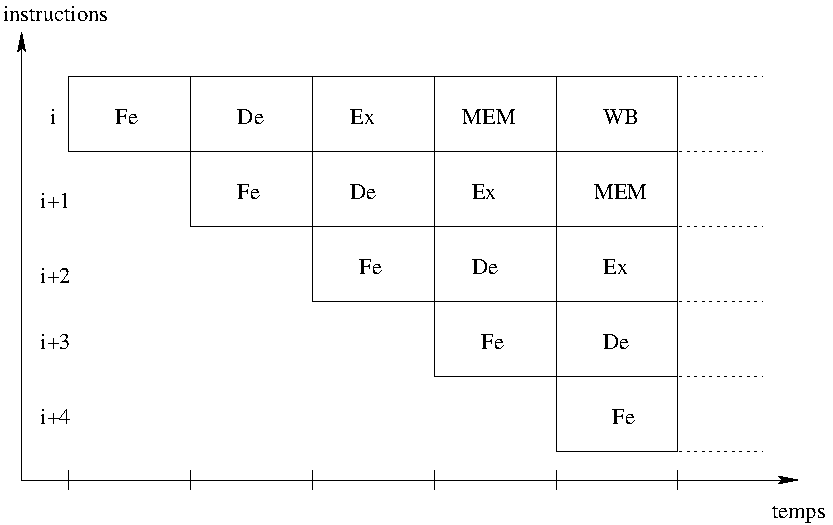
\includegraphics[width=0.8\linewidth]{./images/pipelineDeBase.pdf}
                \caption{Sch�ma de principe d'un pipeline de base � 5 �tages}
                \label{fig:pipelineDeBase}
        \end{center}
\end{figure}

Chaque instruction n�cessite alors id�alement un cycle pour chacune de ces �tapes (cinq cycles dans cet exemple), mais comme une unit� est affect�e pour chaque �tape, autant d'instructions peuvent �tre r�alis�es en m�me temps (soit cinq instructions en m�me temps dans notre exemple). Dans le meilleur des cas, on obtient alors un CPI de 1. Cependant,  certains cas peuvent perturber le pipeline, \emph{les al�as}.

\subsubsection{Diff�rentes cat�gories d'al�as}
\label{sec:pipelineAlea}
Il y a diff�rents cas de figures qui peuvent venir perturber le bon d�roulement du pipeline. Ces al�as ont �t� trait�s en trois cat�gories principales:
\begin{itemize}
\item les \emph{al�as structurels} proviennent d'un manque de ressources. Il n'est pas possible pour le processeur de g�rer correctement le recouvrement des instructions. Par exemple on essaie d'acc�der � de la m�moire � la fois en �criture et en lecture...
\item les \emph{al�as de donn�es} interviennent quand une instruction d�pend du r�sultat de l'instruction pr�c�dente;
\item les \emph{al�as de contr�le} interviennent lors des branchements et des autres instructions qui modifient le compteur programme PC.
\end{itemize}
Il y a alors besoin de g�rer de la mani�re la plus efficace possible ces al�as afin de ne pas retarder le pipeline. En effet, en cas d'al�as, il est n�cessaire d'ins�rer des \emph{bulles} (ou suspensions) afin que le pipeline puisse continuer correctement. Ces suspensions sont autants de cycles perdus.

\subsubsection{Les al�as structurels}
Les al�as structurels sont caus�s par le manque de ressources du processeur.  Un al�a survient par exemple lors du recouvrement des �tapes \texttt{fetch} et \texttt{mem access}. Ici, on a acc�s � la m�moire en lecture pour lire l'instruction suivante, et en lecture ou �criture dans l'�tage \texttt{mem access}. Dans ce cas simple, un recours � deux m�moires cache (\emph{cache instruction} et \emph{cache de donn�es}) permet de d�coupler les deux acc�s. Pour �viter ce genre d'al�as, on utilise g�n�ralement la duplication des ressources, ce qui augmente la quantit� de mat�riel.

\subsubsection{Les al�as de donn�es}
On rencontre dans les al�as de donn�es plusieurs types de d�pendances entre les donn�es. Soit deux instructions \emph{i} et \emph{j} cons�cutives:
\begin{description}
\item[LAE (lecture apr�s �criture):] l'instruction \emph{j} essaie de lire une donn�e avant que l'instruction \emph{i} ne l'ai �crite. C'est le cas le plus courant. (\textsl{RAW: Read After Write} en anglais);
\item[EAE (�criture apr�s �criture):] l'instruction \emph{j} essaie d'�crire une donn�e avant que l'instruction \emph{i} ne l'ait �crite. Les �critures ne se font pas dans le bon ordre. Cet al�a ne se produit que s'il y a plus d'un �tage qui autorise l'�criture, ou en cas d'ex�cution dans le d�sordre.(\textsl{WAW: Write After Write} en anglais);
\item[EAL (�criture apr�s lecture):] l'instruction \emph{j} tente une �criture avant que l'instruction \emph{j} n'ait lu sa donn�e.(\textsl{WAR: Write After Read} en anglais).
\end{description}

Plusieurs recours pour r�duire l'influence des al�as de donn�es sont disponibles, comme des raccourcis mat�riels (ou court-circuits ou d�rivation), une optimisation du compilateur, du renommage de registre, \ldots

\subsubsection{Les al�as de contr�le}
\label{annexe:branchement}
Avec l'utilisation des pipelines, les branchements du programme occasionnent des al�as et ralentissent en cons�quence le fonctionnement du processeur. En effet, lors d'un branchement, les instructions qui ont commenc� � �tre ex�cut�es doivent �tre abandonn�es: il est n�cessaire de suspendre le pipeline (en ins�rant des bulles). En g�n�ral, plus le pipeline est profond et plus le d�lai de branchement en temps de cycles est �lev�. Pour augmenter la vitesse des processeurs, les �tages de pipeline sont de plus en plus courts et les pipelines de plus en plus longs. L' Intel \textsl{Pentium IV} poss�de un pipeline � 20 �tages, soit le double que son pr�d�cesseur le \textsl{Pentium III}.
Plusieurs techniques ont �t� d�velopp�es afin de diminuer au maximum les suspensions relatives aux instructions de saut, en d�tectant les branchement au plus t�t dans le pipeline, en utilisant des algorithmes de pr�dictions de branchement statique ou dynamique combin�s � une ex�cution sp�culative des instructions. 

%%%%%%%%%%%%%%%%%%%%%%%% fin copie.

\subsection{Description et mod�lisation du pipeline simple}
Le comportement temporel des instructions � travers le pipeline est difficile � d�terminer � cause des al�as qui influent dynamiquement sur les latences du pipeline. Il est imp�ratif de prendre en compte ces contraintes lors de l'�laboration d'un simulateur pr�cis au cycle pr�s. 
� partir de la description rapide du principe d'un pipeline dans les sections pr�c�dentes, on peut ajouter les diverses am�liorations qui ont �t� propos�es au cours du temps, am�liorations qui ont pour objectif d'acc�l�rer la vitesse de traitement des instructions (augmentation de la longueur des pipelines par exemple), et aussi de limiter les pertes de performances li�es aux diff�rents al�as. On peut citer par exemple:
\begin{itemize}
\item l'ajout de pr�dicteurs de branchement / ex�cution sp�culative pour limiter les al�as de contr�le;
\item l'ajout de mat�riel pour limiter les al�as structurels;
\item l'utilisation du renommage de registre pour limiter les al�as de donn�es;
\item l'ajout d'unit� fonctionnelles, permettant l'ex�cution parall�le d'instructions (superscalaires) avec ex�cution ordonn�e ou non, ...
\end{itemize}

Ces am�liorations entra�nent une diminution du CPI (Cycles Par Instruction), au d�triment du d�terminisme temporel. Dans tous les cas, on peut se ramener, dans un premier temps, � un pipeline simple, auquel il faudra ajouter un certain nombre de propri�t�s en fonctions des am�liorations � ajouter. %Par exemple, un pipeline superscalaire peut �tre pr�sent� comme un ensemble de pipelines simples interconnect�s qui sont g�r�s de mani�re ind�pendante. Une �tude suppl�mentaire est cependant indispensable pour mod�liser la table de r�servation et le tampon de r�ordonnancement. 

Nous nous int�ressons dans un premier temps � la mani�re de d�crire un pipeline simple, pour aborder dans un deuxi�me temps une mod�lisation de haut niveau, mais temporellement correcte du comportement du pipeline.

\subsubsection{Description du pipeline simple}
\label{sec:descPipeline}
%Dans un premier temps, pipeline simple.
Par la suite, nous nous int�ressons � un pipeline le plus simple possible, lin�aire, de longueur indiff�rente et sans al�a. Nous ajoutons alors des \emph{contraintes temporelles} introduites par les al�as. Nous distinguons deux types de contraintes:
\begin{itemize}
\item les \emph{ressources internes} sont des \emph{contraintes statiques} qui peuvent �tre d�finies statiquement lors d'une premi�re phase d'analyse, pour un instant donn�. Ce genre de contrainte est int�ressant car un certain nombre de calculs peuvent �tre pr�-calcul�s, et n'engendre alors que tr�s peu de charge processeur � l'ex�cution (lors de la simulation);
\item les \emph{ressource externes} sont des \emph{contraintes dynamiques} qui sont d�finies au cours de la simulation, soit parce qu'elles sont d�pendantes des donn�es, soient parce qu'elles inter-agissent avec d'autres composants concurrents (le contr�leur m�moire est un exemple).
\end{itemize}

\paragraph{Ressource interne}
Les ressource internes sont principalement utilis�es pour mod�liser les al�as structurels. Comme le champ de ces ressources est limit� aux contraintes qui sont compl�tement sous le contr�le du pipeline, seules les instructions qui sont dans le pipeline peuvent \emph{prendre} ou \emph{relacher} une ressource interne. 

Quand l'�tat du pipeline est connu (\cad que les instructions pr�sentes dans chaque �tage de pipeline sont d�finies), alors l'�tat de chaque ressource interne est compl�tement d�fini (\emph{prise} ou \emph{relach�e}). 

Par exemple, chaque �tage de pipeline est mod�lis� sous la forme d'une ressource interne. D�s qu'une instruction entre dans un �tage, elle prend la \emph{ressource interne} associ�e. Elle relache cette ressource lorsqu'elle quitte l'�tage. La contrainte ajout�e dans notre description du pipeline est alors que \emph{chaque �tage de pipeline peut contenir au plus une seule instruction}. 

\paragraph{Ressource externe}
Les ressources externes sont utilis�es pour d�crire les ressources qui sont \emph{partag�es} avec d'autres composants mat�riels qui �voluent concurremment, comme un \textsl{timer} ou un contr�leur m�moire. Les ressources externes sont alors une extension des \emph{ressources internes} pour d�crire des \emph{contraintes dynamiques}. Par exemple, avec un contr�leur de m�moire, le pipeline est bloqu� s'il fait une requ�te au contr�leur et que celui-ci est occup� (par un autre processeur par exemple, ou un DMA, ...). Si le contr�leur m�moire est disponible, l'�tage de pipeline qui a fait la requ�te peut alors prendre la ressource.

Si une ressource externe peut �tre prise par une instruction dans plus d'un �tage de pipeline, une priorit� est mise en place entre les �tages. Par exemple, deux �tages de pipeline peuvent �tre en comp�tition pour un acc�s m�moire sur un micro-contr�leur avec un pipeline simple, sans cache de donn�e et d'instruction.

\paragraph{Instructions}
Au niveau de la description du pipeline, les instructions peuvent �tre regroup�es suivant lors comportement temporel. Ceui-ci est directement li� aux ressources qui vont �tre prises et rel�ch�es au cours de l'execution de ces instructions dans les diff�rents �tages de pipeline. Ainsi les instructions qui utilisent les \emph{m�me ressources} (internes et externes) sont regroup�es pour former des \emph{classes d'instructions}. Ceci n'est pas du tout en rapport avec les instruction qui ont un \emph{comportement} proche. Par exemple les instructions \texttt{ADD Rd, Rs1, Rs2} et  \texttt{AND Rd, Rs1, Rs2} utilisent les m�mes ressources (acc�s m�moire, ALU) et sont par cons�quent dans la m�me classe d'instruction, cependant, leurs comportements sont diff�rents.


\subsubsection{Mod�lisation du pipeline simple sous forme d'automates d'�tat finis}
La description qui a �t� pr�sent�e ici est fortement li�e au mod�le sous jacent utilis� pour la simulation, c'est pourquoi une introduction du mod�le de pipeline est pr�sent� ici, afin de mieux aborder les notions de ressource internes et externes pr�sent�es dans la section pr�c�dente.

\paragraph{Int�r�t}
La mod�lisation du pipeline simple qui a �t� choisie est celle des \emph{automates d'�tats finis}. L'utilisation d'automates pour la mod�lisation des pipelines a plusieurs avantages:
\begin{itemize}
\item certaines contraintes sont r�solues au moment de la g�n�ration de l'automate, \cad au moment de la g�n�ration du simulateur. Cette propri�t� int�ressante signifie que des calculs sont effectu�s une fois pour toute, sans ralentir ensuite la simulation;
\item la transformation d'un automate en code ex�cutable est particuli�rement efficace. Au niveau du code g�n�r�, passer d'un �tat � un autre revient � lire une valeur dans une table, ce qui est tr�s rapide, contrairement � d'autres mod�les comme les r�seaux de Petri;
\item Le temps d'acc�s au prochain �tat de l'automate est en temps constant, et ainsi la vitesse de simulation de l'automate n'est pas d�pendante du nombre d'�tats de l'automate. Ceci reste toutefois � relativiser avec l'utilisation de la m�moire cache de la machine h�te.
\end{itemize}

\paragraph{Des �tats}
Un �tat de l'automate repr�sente l'�tat du pipeline � un cycle donn�, comme l'illustre la figure \ref{fig:pipelineState}.
\begin{figure}		%% �tat d'automate.
  \begin{center}
    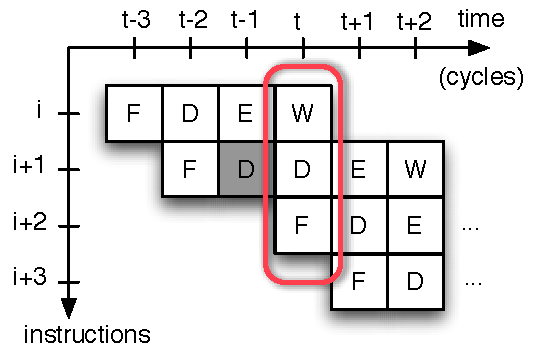
\includegraphics[width=0.6 \linewidth]{./images/pipelineState.pdf}
    \caption{Un �tat de l'automate repr�sente l'�tat du pipeline � une date donn�e. Dans cet exemple avec un pipeline � 4 �tages (F-D-E-W), 3 instructions sont dans le pipeline, et l'�tage E a une suspension � la date {\sl t}.}
    \label{fig:pipelineState}
  \end{center}
\end{figure}
L'automate repr�sente alors l'ensemble des scenarios possibles d'ex�cutions. Un �tat de l'automate est repr�sent� par la liste de toutes les paires (classe d'instruction, �tage de pipeline) dans le pipeline � un instant donn�. Pour un syst�me avec $c$ classes d'instructions, il y a alors $c+1$ cas possibles pour chaque �tage $e$ de pipeline (chaque classe d'instruction, ou une suspension). L'automate est alors fini, car il y a au plus $(c+1)^{e}$ �tats. L'�tat initial est celui qui repr�sente un pipeline vide.

Par exemple, sur un mod�le bas� sur le jeu d'instruction du co-processeur RISC XGate du STAR12X  de FreeScale \cite{xgateUserMan}, avec un pipeline de 6 �tages, 5 classes d'instructions sont n�cessaires seulement (il y a 3 ressources externes). il y a donc au plus $46656$ �tats\footnote{La vraie architecture du co-processeur n'est compos�e que de 2 �tages, et il n'y aurait que 36 �tats dans l'automate.}.

\paragraph{Et des transitions}
Une transition est franchie � chaque cycle d'horloge. Une transition d�pend uniquement de:
\begin{itemize}
\item l'�tat des ressources externes (prises ou non);
\item la classe de la prochaine instruction qui va entrer dans le pipeline;
\end{itemize}

Un int�r�t majeur de cette approche r�side dans le fait que les ressources internes, du fait de leur caract�re statique, sont r�solues directement au niveau de la g�n�ration de l'automate. Elles n'apparaissent par cons�quent pas dans l'�valuation de la transition. Cette condition de transition (�tat des ressources externes et prochaine classe d'instruction) est appel�e \emph{condition de transition basique}. Comme plusieurs conditions peuvent appara�tre pour aller d'un �tage � un autre, la condition de transition globale est alors une disjonction des conditions de transition basiques. 

Le nombre de transitions est limit� au maximum � $c \times 2^{R_{ext}}$ pour chaque �tat (o� $R_{ext}$ est le nombre de ressources externes). Il y a donc au plus $(c+2)^{e} \times 2^{R_{ext}}$ transitions pour l'automate entier. 

Pour notre exemple bas� sur un co-processeur XGate et une architecture � 6 �tages, on obtient alors 40 transitions possibles par �tats ($5 \times 2^{3}$). 

La g�n�ration de l'automate sort du cadre de ce document, mais � fait l'objet d'une soumission � la conf�rence DATE'07 (Design, Automation and Test in Europe) � Nice. Certains probl�mes apparaissent avec l'utilisation des automates, comme l'explosion combinatoire du nombre d'�tats lors de la g�n�ration quand la complexit� du mod�le devient importante. Le nombre d'�tats cro�t en effet exponentiellement en fonction de la taille du pipeline, et polynomialement en fonction du nombre de classes d'instruction. Ces probl�mes sont actuellement envisag�s, en optimisant d'une part les calculs et en r�duisant la taille des automates, et en �valuant d'autre part la possibilit� de couper un pipeline en 2 pipelines de plus faible longueur pour obtenir 2 automates plus petits.

% � mettre dans la partie automata.
%\subsection{Une exemple: r�solution des al�as de donn�es}
%Par la nature dynamique des ressources externes, une propri�t� int�ressante est la possibilit� de v�rifier les al�as de donn�es. On utilise alors un \emph{contr�leur de d�pendance des donn�es}, auquel est associ� une ressource externe. Supposons par exemple ici que les 2 premiers �tages du pipeline soit l'�tage \texttt{fetch}, suivi par l'�tage \texttt{decode} qui lit les op�randes. L'interaction entre le \emph{contr�leur de d�pendances de donn�es} et l'instruction est pr�sent� dans l'algorithme \ref{algo:dataDep}: Une instruction qui est dans l'�tage \texttt{Fetch} envoie une \emph{requ�te} au contr�leur pour v�rifier de la disponibilit� des op�randes. Si au moins une op�rande n'est pas disponible, la ressource externe associ�e passe � l'�tat \texttt{non disponible}. Lors de 

%\begin{algorithm}
%	\eIf{il y a une instruction dans l'�tage Fetch \textbf{and} Cette instruction aura besoin d'op�randes dans l'�tage Decode}{
%			- L'instruction envoie une requ�te au contr�leur\;
%			\eIf{Si au moins une op�rande n'est pas disponible}{
%				- la requ�te �choue: la ressource externe associ�e passe � l'�tat  \texttt{non disponible})\;
%			}{
%				- la requ�te est valid�e: la ressource externe associ�e passe � l'�tat \texttt{disponible})\;\;
%			}
%	}{
%		- la requ�te est valid�e: la ressource externe associ�e passe � l'�tat \texttt{disponible})\;
%	}	
%	\label{algo:dataDep}
%	\caption{Interaction entre le contr�leur de d�pendance de donn�es et une instruction durant la simulation.}
%\end{algorithm}		 

\subsection{Mapping des instructions sur les ressources mat�rielles}
La relation entre les instructions et les ressources mat�rielles utilis�es est int�gr�e au niveau de la description; cependant, comme il a �t� pr�cis� dans la section \ref{chap:jeuInstruction}, le jeu d'instruction est ind�pendant de la micro-architecture. Cette contrainte est r�solue en associant les \emph{op�rations} r�alis�es par les instructions avec les �tages de pipeline. Il est alors du ressort du compilateur de d�couper le comportement de chaque instruction � travers les diff�rents �tages du pipeline. 

Consid�rons par exemple l'op�ration d'addition: ADD Rd,Rs1,Rs2 qui pourrait �tre d�crite de la mani�re suivante\footnote{\texttt{u16} correspond � une variable non sign�e sur 16 bits}:
\begin{verbatim}
u16 a := gprRead(Rs1); 
u16 b := gprRead(Rs2); 
u16 c := a+b;
updateFlagRegisters(a,b,c);
u16 gprWrite(Rd, c); 
\end{verbatim}
Le code\footnote{L'�tape de r�cup�ration de l'instruction, et de d�codage n'est pas pr�sente, dans un souci de simplicit�} pr�sent� pourrait correspondre au code de l'ADL, apr�s une premi�re �tape d'analyse, charg� d'expanser chaque instruction, o� Rs1, Rs2 et Rd sont les num�ros de registres qui sont fournis par la vue binaire de l'instruction (voir section \ref{sec:vueBinaire}). Le code de l'instruction ne prend aucune information en provenance de l'architecture interne. Consid�rons maintenant une architecture pipelin�e bas�e sur une architecture RISC, � 5 �tages (comme l'architecture DLX dans \cite{HennessyPatterson}):
\begin{description}
\item[Fetch] Le code de l'instruction est r�cup�r� � partir du cache d'instruction;
\item[Decode] Le code de l'instruction est d�cod�, les conditions de saut sont r�solues, les op�randes sont lues;
\item[Execute] Le op�rations de l'ALU sont effectu�es;
\item[Memory] Les acc�s m�moires sont r�alis�s;
\item[Write Back] Les op�randes de r�sultats sont �crits.
\end{description}

� partir du mod�le pr�sent�, on associe � chaque �tage de pipeline un certain nombre d'op�rations possibles. Dans notre exemple, les op�rations seront:
\begin{itemize}
\item l'appel � gprRead ne peut �tre r�alis� que dans l'�tage \texttt{Decode};
\item l'op�ration '+' ne peut �tre r�alis�e que dans l'ALU, qui est dans l'�tage \texttt{Execute};
\item la mise � jour du registre d'�tat est r�alis�e dans l'ALU, qui est dans l'�tage \texttt{Execute};
\item l'op�ration gprWrite ne peut �tre r�alis�e que dans l'�tage \texttt{Write Back}.
\end{itemize}
On introduit alors dans le langage la notion de \texttt{resource} (� ne pas confondre avec les ressources internes et externes de la section \ref{sec:descPipeline}), qui permet de faire le lien entre une op�ration, et l'�tage de pipeline associ�. 


Il s'ensuit que l'instruction sera \emph{mapp�e} sur l'architecture interne comme le montre la figure \ref{fig:mappingInst}.
\begin{figure} [h]
        \begin{center}
                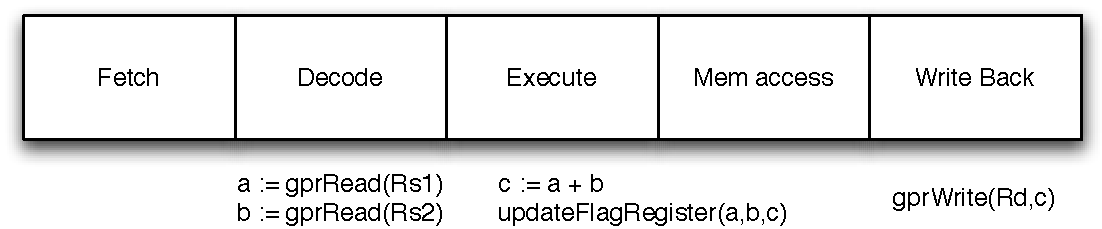
\includegraphics[width=0.8\linewidth]{./images/mappingInst.pdf}
                \caption{Exemple de mapping de l'instruction ADD sur un pipeline � 5 �tages.}
                \label{fig:mappingInst}
        \end{center}
\end{figure}

Avec une telle architecture, le comportement des instruction est compl�tement dissoci� du mod�le de l'architecture mat�rielle sous jacente. Par cons�quent, il est tout � fait envisageable, � partir d'un unique jeu d'instruction, de proposer plusieurs architectures internes, il sera n�cessaire de modifier le \emph{mapping} des op�rations r�alis�es par le jeu d'instruction sur la nouvelle architecture interne. C'est le cas par exemple des processeurs ARM, dont les diff�rente familles utilisent le m�me jeu d'instruction, mais bas� sur des tailles de pipeline diff�rentes. %� v�rifier: �tre plus pr�cis.

\subsection{Hi�rarchie m�moire}
\label{sec:mem}
%probl�matique des caches. Influence importante sur le comportement. Mod�le de cache. Cependant, les mod�les de caches sont g�n�ralement peu diff�rents, et leur mod�lisation � partir d'un squelette para�t envisageable. 
La hi�rarchie m�moire est un m�canisme qui influe aussi dans une large mesure sur le comportement temporel d'un processeur. Cependant, la description de la hi�rarchie m�moire para�t plus simple que l'architecture interne du processeur:
\begin{itemize}
\item la hi�rarchie m�moire n'influe sur le reste du syst�me que par le blocage sur un acc�s m�moire, ce qui est d�j� pris en compte dans le mod�le du pipeline (� travers les ressources externes);
\item il existe des politiques de cache classiques (LRU, Random, ..) qui seront certainement directement int�gr�es dans le compilateur, sous la forme de squelette par exemple.
\item les param�tres d'un bloc m�moire peuvent directement �tre int�gr�s dans un mod�le g�n�ral de bloc m�moire (taille, largeur de bus, acc�s en rafale (burst), latence en lecture, en �criture).
\end{itemize}
Il devra �tre toutefois possible de d�crire, sous forme algorithmique le comportement d'une politique d'allocation de caches.
\section{Conclusion}

Les objectifs du langages ont �t� bien identifi�s, tant sur la partie jeu d'instruction, que la mod�lisation interne d'un pipeline simple. 

Au niveau du jeu d'instruction, les bases du langages ont �t� d�finies et la description de plusieurs processeurs (ARM et XGate pour l'instant) a �t� r�alis�e. Il sera certainement n�cessaire d'enrichir encore le langage pour d'autre architectures. les outils sont actuellement en cours de d�veloppement, avec pour premier objectif de g�n�rer un simulateur de jeu d'instruction � partir de la description. Il faudra, dans un deuxi�me temps, interfacer cet outil avec le mod�le de l'architecture interne. 

Au niveau de l'architecture interne, deux outils permettant la g�n�ration de code � partir de la description d'un pipeline simple ont �t� d�velopp�: un premier permettant de g�n�rer le mod�le du pipeline sous la forme d'un automate � partir de la description (\emph{p2a}), et un second qui g�n�re le code source du mod�le du pipeline � partir de l'automate (\emph{a2cpp}). Ces outils ont permis de valider l'approche par automate. Il est maintenant n�cessaire d'enrichir les descriptions pour pouvoir mod�liser des processeurs plus complexes (superscalaires, avec ex�cution ordonn�e ou non), d'aborder la mod�lisation hi�rarchie m�moire, ainsi que les composants externes (timers, I/O, ...).


\bibliographystyle{plain}
\bibliography{hadl}


\end{document}